% !TEX root = ../main.tex
\chapter{IoT Brain} \label{ch:framework}

This chapter is going to give some informations about the design choice taken while implementing the approaches in \textbf{\autoref{ch:model}} and \textbf{\autoref{ch:diagnosis}}. Implementation efforts were aimed at providing a further degree of scalability to the approach and leveraging cloud based technologies as well as reducing the technicality of the involved resource.
It will be presented a use case that shows the % TODO explain why this framework can help in spreading a EMS

\section{IoT BRAIN and KITT}
IoT Big scale Reasoning and Analytic INsights (IoT BRAIN) allows to specify semantic models for IoT systems and run analytics across them automatically. Its core is the light-weight knowledge framework named Knowledge Inference Technology for IoT (KITT) that provides a simple API to model, manage and reason on the semantic knowledge model. It is split in multiple layers of different abstraction level that base on a common semantic modeling strategy.
This architecture implements the concepts explained in the previous chapters with a strong emphasis on the scalability and availability of the approach.

\begin{figure}
  \centering
  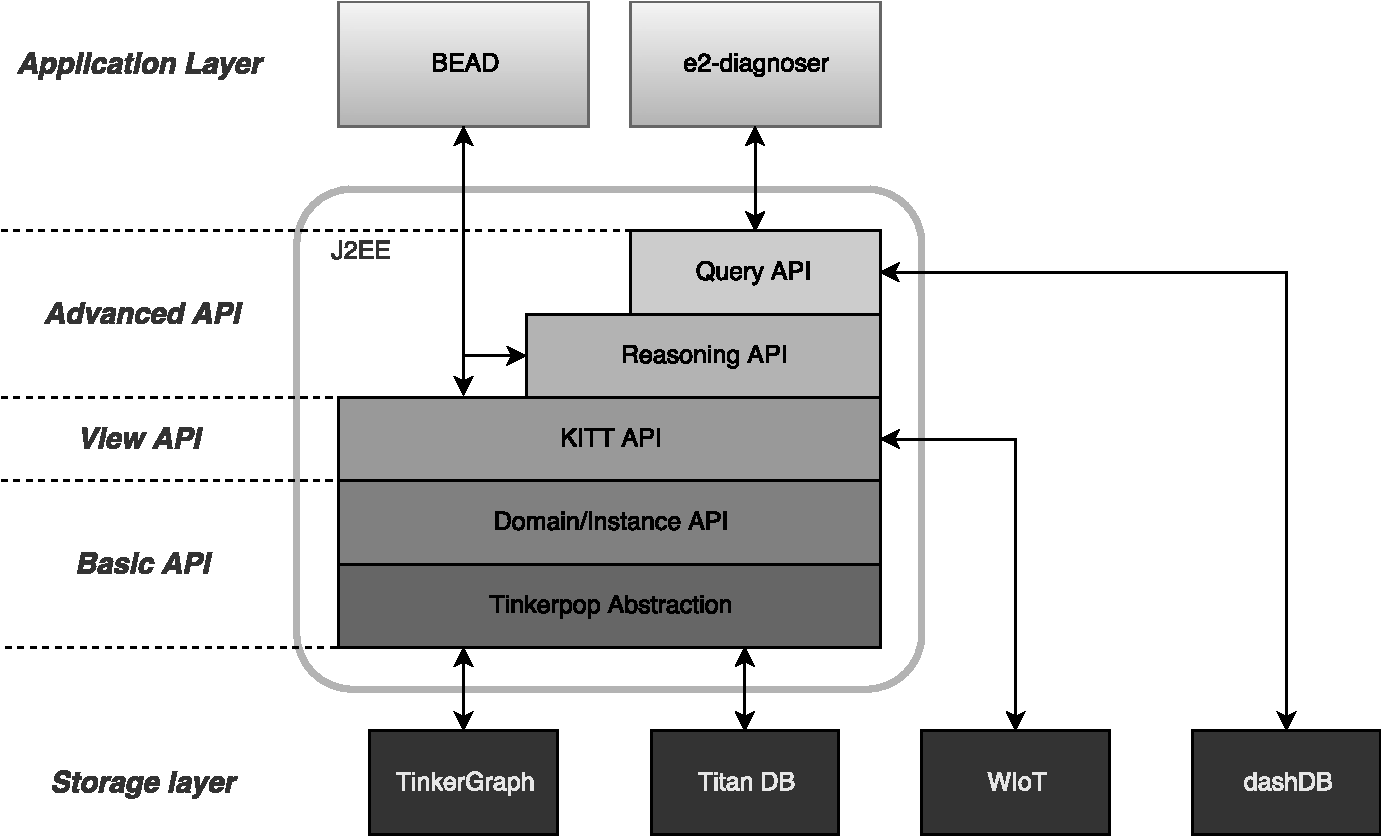
\includegraphics[width=1\textwidth]{iot_brain.pdf}
  \caption{IoT BRAIN architecture}
  \label{fig:iot_brain}
\end{figure}

IoT BRAIN, which architecture is shown in \autoref{fig:iot_brain}, is built upon a storage layer that is comprised of a graph database, used for storing the semantic model of the building. The Watson IoT platform allows easy connection and dispatch of
data securely to the cloud using the open, lightweight MQTT messaging protocol. The storage layer is completed by a dashDB, an SQL database that provides efficient storage of time series and high query performance.
On top of this layer sits the core of the project which realize the theoric process shown in \autoref{fig:approach_overview}.

\subsection{Graph database vs. RDF Store}
why graphDB:
cloud
property centric
need to evolve SPARQL
